\graphicspath{{chapter_4}}
\chapter[Self-supervised Laparoscopic Camera Motion Prediction]{Self-supervised Laparoscopic Camera Motion Prediction for Imitation Learning}
\chaptermark{Camera Motion Prediction}
\label{chap:camera_motion_prediction}
\minitoc

\paragraph{Disclaimer} This \chapref{chap:camera_motion_prediction} is an \textit{in extenso} reproduction of~\cite{huber2023deep}. Only \secref{c4:sec:introduction} was altered to highlight additional context within the scope of this thesis.

\newpage

\section{Introduction}
\label{c4:sec:introduction}
In the previous \chapref{chap:camera_motion_extraction}, it was demonstrated that the hypothesized supervised laparoscopic camera motion extraction from \figref{in:fig:camera_motion} indeed outperforms classical means of extraction, see \figref{c3:fig:resnet34_c} and \figref{c3:fig:qualitative}. This was achieved through a novel data augmentation step, refer \figref{c3:fig:hom}. In fact, the introduced method proved so robust that it outperformed classical methods on \gls{mis} data, although it was trained on \gls{rmis} data, see \figref{c3:fig:qualitative}. This is necessary for extracting homographies from \gls{mis} data, i.e. non-robotic data, and to imitate a handheld laparoscope's motion. The extracted homography, i.e. action $\hat{a}^*_t$, refer \figref{in:fig:hypothesized_pipeline}, could already be combined with the proposed visual servo scheme from \chapref{chap:robotic_endoscope}, however, this would ignore that the surgical scene changes over time (temporality assumption) as was mentioned in \secref{c2:sec:introduction}.

In this chapter \chapref{chap:camera_motion_prediction}, we will finally investigate how the extracted homographies can be utilized in a self-supervised training scheme to implement the \gls{il} for predicting desired actions $\hat{a}^*_t$ from image states $\hat{s}_t$, see \figref{in:fig:hypothesized_pipeline}. This builds on the realization that camera motion is intrinsic to videos of laparoscopic interventions and that camera motion can be harvested from them, as was already discussed in \secref{in:sec:supervised_self_supervised}. Since no public dataset exists for state-action pairs, some work continues to focus on the tools to infer camera motion~\cite{li2021data}, or learns on a robotic setup altogether~\cite{li20223d} where camera motion is accessible. In this chapter, we address those shortcomings, to enable \gls{il} on large scale datasets of retrospective laparoscopic surgery videos.

% Automation in robot-assisted minimally invasive surgery (RMIS) may reduce human error that is linked to fatigue, lack of attention and cognitive overload~\cite{fiorini2022concepts}.
% It could help surgeons operate such systems by reducing the learning curve~\cite{van2018learning}.
% And in an ageing society with shrinking workforce, it could help to retain accessibility to healthcare. It is therefore expected that parts of RMIS will be ultimately automated~\cite{davenport2019potential,zidane2023robotics}. On the continuous transition towards different levels of autonomy, camera motion automation is likely to happen first~\cite{kitaguchi2022artificial}.

% Initial attempts to automate camera motion in RMIS include rule-based approaches that keep surgical tools in the center of the field of view~\cite{da2020scan,garcia2022robotic,sandoval2021towards}. The assumption that surgical tools remain centrally is, however, simplistic, as in many cases the surgeon may want to observe the surrounding anatomy to decide their next course of action. 

% Contrary to rule-based approaches, data-driven methods are capable to capture more complex control 
%modes.
%policies.
%Example data-driven methods suitable for camera motion automation include reinforcement learning (RL) and imitation learning (IL). The sample inefficiency and potential harm to the patient currently restrict \gls{rl} approaches to simulation~\cite{su2021multicamera,scheikl2023lapgym,agrawal2018automating}, where a domain gap remains. Work to bridge the domain gap and make \gls{rl} algorithms deployable in real setups have been proposed~\cite{cartucho2021visionblender,marzullo2021towards}, but clinical translation has not yet been achieved. For \gls{il}, on the other hand, camera motion automation could be learned from real data, thereby implicitly tackling the domain-gap challenge. The downside is that sufficient data may be difficult to collect. Many works highlight that lack of expert annotated data hinders progress towards camera motion automation in RMIS~\cite{maier2022surgical,kassahun2016surgical,esteva2019guide}.
%To this end, it 
% It is thus not surprising that existing literature on \gls{il} for camera motion automation utilizes data from mock setups~\cite{ji2018learning,wagner2021learning}.

% Recent efforts to make vast amounts of laparoscopic intervention videos publicly available~\cite{maier2022surgical} drastically change how \gls{il} for camera motion automation can be approached. So far, this data is leveraged mainly to solve auxiliary tasks that could contribute to camera motion automation. As reviewed in~\cite{loukas2018video}, these tasks include tool and organ segmentation, as well as surgical phase recognition. 


\subsection{Contributions}
We build on \chapref{chap:camera_motion_extraction} for computationally efficient state-action pair extraction from publicly available datasets of laparoscopic interventions, which yields more than $20\times$ the amount of data that was used in the closed source data of~\cite{li2022learning}. To our best knowledge, this dataset marks the largest and only state-action pair dataset for laparoscopic camera motion \gls{il}. On top of the sheer amount of additional data, we extract homography estimates at runtime, de facto generating data on the fly. Contrary to~\cite{li2022learning}, our camera motion extraction does not rely on image features, which are sparse in surgical videos, and is intrinsically capable to differentiate between camera and object motion. We further propose a novel importance sampling and data augmentation step for achieving camera motion automation \gls{il} in this chapter. It is indeed the importance sampling, which renders learning to predict motion feasible.

%21x

%~170 minutes their
%~2950 minutes cholec80
%~630 minutes heichole

% ~\cite{huber2022deep}
% ~\cite{huber2021homography}

% Minimally invasive robot assisted surgery leads to reduced patient pain, reduced blood loss, shorter recovery times, less scarring, and reduced risk of infection ~\cite{}. Additionally, it offers surgeons better ergonomics that lead to reduced fatigue, greater precision, and less physical exertion ~\cite{}. On the downside, however, it requires additional training.

% make clear that camera motion is the target

% Efforts have been made to reduce training requirements for surgeons by improved human-machine interfaces, e.g. through voice, gaze, or the introduction of haptic devices ~\cite{}. The effort is to essentially relieve surgeons of some of their tasks, similar to what an assistant would do, through robot autonomy.


%\textbf{This is all a bit too sudden. I think you need to make the case for autonomous endoscope motion, how you will extract motion, and why this is important. Also, what have others done on the topic? Your introduction is a bit too general. Keep what you have, but slowly narrow it down to something more specific. You are solving a very specific problem, not the full imitation learning problem}

% dive deeper into homography estimation / prediction
% used for visual servoing, shown to work in the surgical context

\section{Materials and Methods}
The proposed approach to learning camera motion prediction is summarized in \figref{c4:fig:training_pipeline}. The following sections will describe its key components in more detail.

% \begin{landscape}
\begin{figure}[htb]
\centering
%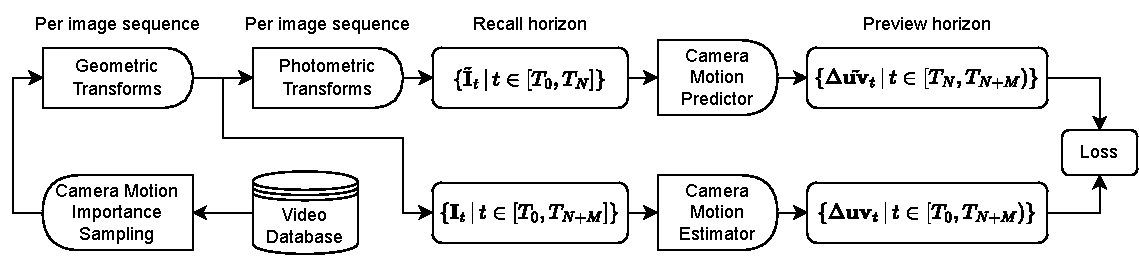
\includegraphics[width=0.7\paperheight]{fig/23_02_13_miccai_figures.drawio.pdf}
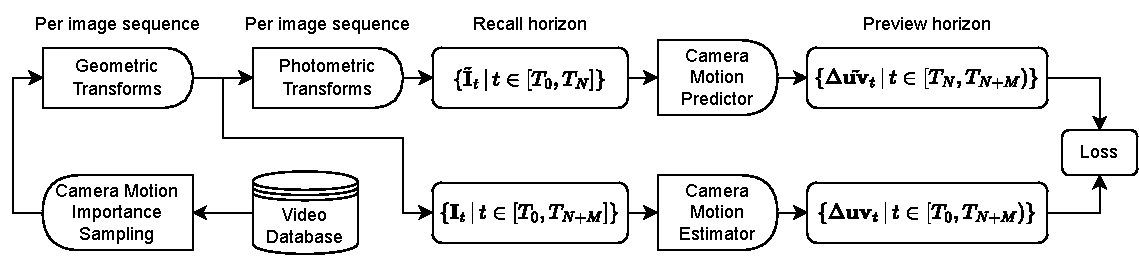
\includegraphics[width=\textwidth]{fig/23_02_13_miccai_figures.drawio.pdf}
\caption{Training pipeline, refer to  \secref{c4:sec:proposed_pipeline}. From left to right: Image sequences are importance sampled from the video database and random augmentations are applied per sequence online. The lower branch estimates camera motion between subsequent frames, which is taken as pseudo-ground-truth for the upper branch, which learns to predict camera motion on a preview horizon.}
\label{c4:fig:training_pipeline}
\end{figure}
% \end{landscape}


\subsection{Theoretical Background}
\label{c4:sec:theoretical_background}
Points on a plane, as observed from a moving camera, transform by means of the $3\times3$ projective homography matrix $\mathbf{G}$ in image space, see \secref{in:sec:homography_based_camera_motion_formulation}. Thus, predicting future camera motion (up to scale) may be equivalently treated as predicting future projective homographies.

It has been shown in~\cite{detone2016deep} that the four point representation of the projective homography, \emph{i.e.,}  taking the difference between four points in homogeneous coordinates $\Delta\mathbf{uv} = \{\mathbf{p}_i - \mathbf{p}^\prime_i\,|\,i \in [0, 4)\} \in \mathbb{R}^{4\times2}$ that are related by $\mathbf{G}\mathbf{p}_i \sim \mathbf{p}^\prime_i\,\,\forall i$, is better suited for deep learning applications than the $3\times3$ matrix representation of a homography, which is harder to estimate correctly.
%
Therefore, in this work, we treat camera motion $\mathcal{C}$ as a sequence of four point homographies on a time horizon $[T_0, T_{N+M})$, $N$ being the recall horizon's length, $M$ being the preview horizon's length. Time points 
%$T_i$
lie $\Delta t$ apart, that is $T_{i+1} = T_{i} + \Delta t$. For image sequences of length $\text{N+M}$,
we work with
four point homography sequences $\mathcal{C}=\{\Delta\mathbf{uv}_t \,|\, t\in[T_0, T_{N+M})\}$.



\subsection{Data and Data Preparation}
\label{c4:sec:data_and_data_preparation}
Three datasets are
%acquired
curated
to train and evaluate the proposed method: two cholecystectomy datasets (laparoscopic gallbladder removal), namely Cholec80~\cite{twinanda2016endonet} and HeiChole~\cite{wagner2023comparative}, and one hysterectomy dataset (laparoscopic uterus removal), namely AutoLaparo~\cite{wang2022autolaparo}.

% The laparoscope typically captures a circular field of view, with status indicators often displayed on the image borders. Further, reflected light frequently exposes parts of the covered regions. 

To remove status indicator overlays from the laparoscopic videos, which may hinder the camera motion estimator, we identify the bounding circle of the circular field of view using~\cite{Budd2022RapidDataset}. We crop the view about the center point of the bounding circle to a shape of $240\times320$, so that no black regions are prominent in the images.

% The split is done on a video basis, \emph{e.g.,} be dataset $\text{A} = \{\text{vid}_0, \text{vid}_1, \text{vid}_2, \text{vid}_3\}$, then a possible split is $\text{A}_\text{training} = \{\text{vid}_0, \text{vid}_1\}$, $\text{A}_\text{validation} = \{\text{vid}_2\}$, and $\text{A}_\text{testing} = \{\text{vid}_3\}$. In other words, there is never an overlap. 

All three datasets are split into training, validation, and testing datasets. We split the videos by frame count into $80\pm 1\,\%$ training and $20 \pm 1\,\%$ testing. Training and testing videos never intersect. We repeat this step to further split the training dataset into (pure) training and validation datasets.

Due to errors during processing the raw data, i.e. failure to detect the bounding circle automatically, we exclude videos $19$, $21$, and $23$ from HeiChole, as well as videos $22$, $40$, $65$, and $80$ from Cholec80. This results in dataset sizes of: Cholec80 - $4.4e6$ frames at $25\,\text{fps}$, HeiChole - $9.5e5$ frames at $25\,\text{fps}$, and AutoLaparo - $7.1e4$ frames at $25\,\text{fps}$.

% cholec80 frames: 4422770
% heichole frames: 948929
% phantom frames: 7180
% autolaparo frames: 70590

\subsection{Proposed Pipeline}
\label{c4:sec:proposed_pipeline}

% previously in figure c4:fig:training_pipeline, double check
% Image sequences are loaded from a video database and geometric transforms, i.e transforms that flip the images / manipulate the perspective and so on, are applied equally to each image within the sequence. The pipeline is then split into two branches. One for camera motion estimation and one for the camera prediction. No further transforms are applied to the camera motion estimation branch to guarantee optimal estimation. Additional photometric transforms, i.e transforms that modify the contrast / color temperature / noise and so on, are applied to the camera motion prediction branch for further augmentation. The estimator takes as input the entire image sequence and estimates camera motion between subsequent frames. The predictor takes as input a recall horizon of past images and predicts a preview horizon of future camera motion. The predictor is optionally conditioned on previous camera motion from the recall horizon. Finally, a loss is computed between estimated and predicted motion.

\subsubsection{Video Database and Importance Sampling}
\label{c4:sec:video_database_and_importance_sampling}
The curated data from \secref{c4:sec:data_and_data_preparation} is accumulated into a video database. Image sequences of length $N+M$ are sampled at a frame increment of $\Delta n$ between subsequent frames and with $\Delta c$ frames between the sequence's initial frames. Prior to adding the videos to the database, an initial offline run is performed to estimate camera motion $\Delta\mathbf{uv}$ between the frames. This creates image-motion correspondences of the form $(\mathbf{I}_n\,,\mathbf{I}_{n+\Delta n}\,,\Delta\mathbf{uv}_n)$. Image-motion correspondences where $\mathbb{E}(||\Delta\mathbf{uv}_n||_2) > \sigma$, with sigma being the standard deviation over all motions in the respective dataset, define anchor indices $n$. Image sequences are sampled such that the last image in the recall horizon lies at index $n = N-1$, marking the start of a motion. The importance sampling samples indices from the intersection of all anchor indices, shifted by $-N$, with all possible starting indices for image sequences.

\subsubsection{Geometric and Photometric Transforms}
\label{c4:sec:geometric_and_photometric_transforms}
The importance sampled image sequences are fed to a data augmentation stage. This stage entails geometric and photometric transforms. The distinction is made because downstream, the pipeline is split into two branches. The upper branch serves as camera motion prediction whereas the lower branch serves as camera motion estimation, also refer to the next section.
As it acts as the source of pseudo-ground-truth,
it is crucial that the camera motion estimator performs under optimal conditions, hence no photometric transforms, i.e. transforms that change brightness / contrast / fog etc., are applied. Photometrically transformed images shall further be denoted as $\tilde{\mathbf{I}}$. To encourage same behavior under different perspectives, geometric transforms are applied, i.e. transforms that change orientation / up to down / left to right etc. Transforms are always
%to be
sampled randomly, and 
%to be
applied consistently to the entire image sequence.
% maybe cite imgaug
 
\subsubsection{Camera Motion Estimator and Predictor}
\label{c4:sec:camera_motion_estimator_and_predictor}
The goal of this work is to have a predictor learn camera motion computed by an estimator.
The predictor takes as input a photometrically and geometrically transformed recall horizon $\{\tilde{\mathbf{I}}_t\,|\,t\in[T_0, T_N)\}$ of length $N$, and predicts camera motion $\tilde{\mathcal{C}} = \{\Delta \tilde{\mathbf{uv}}_t\,|\,t\in[T_N,T_{N+M})\}$ on the preview horizon of length $M$. The estimator takes as input the geometrically transformed preview horizon $\{\mathbf{I}_t\,|\,t\in[T_M, T_{N+M})\}$ and estimates camera motion $\mathcal{C}$, which serves as a target to the predictor. The estimator is part of the pipeline to facilitate on-the-fly perspective augmentation via the geometric transforms.

% maybe adjust figure so estimator only inputs preview horizon

% make this part of results????
% cite feature-based ie loftr, surf, sift / and end-to-end
% also mention downside of end-to-end, that is large homographies
% talk about runtime, memory footprint, accuracy, object motion, texture
% mention predictor architecture

% feature-based homography estimators: de-stabalize training (outliers), slow
% autolaparo misses rotation case, generally doesn't de-couple cases well
% 4 dof can be classified through 4 cases (cross)

\section{Experiments and Evaluation Methodology}
The following two sections elaborate the experiments we conduct to investigate the proposed pipeline from \figref{c4:fig:training_pipeline} in \secref{c4:sec:proposed_pipeline}. First the camera motion estimator is investigated, followed by the camera motion predictor.
%Since the camera motion estimator was studied in detail in~\cite{huber2022deep}, the main focus of this work shall lie on the camera motion predictor. However, since there exists no data on camera motion distribution in videos of laparoscopic interventions, 
% a brief experiment is dedicated to determine camera motion distribution in videos of laparoscopic interventions.
%This section shall also probe the camera motion estimator for the purpose of online camera motion estimation.

\subsection{Camera Motion Estimator}
\label{c4:sec:camera_motion_estimator}
\subsubsection{Camera Motion Distribution} 
To extract the camera motion distribution, we run the camera motion estimator of \chapref{chap:camera_motion_extraction} with a ResNet-34 backbone over all datasets from \secref{c4:sec:data_and_data_preparation}. We map the estimated four point homographies to up/down/left/right/zoom-in/zoom-out for interpretability. Left/right/up/down corresponds to all four point displacements $\Delta\mathbf{uv}$ consistently pointing left/right/{\allowbreak}up/down respectively.
Zoom-in/out corresponds to all four point displacements $\Delta\mathbf{uv}$ consistently pointing inwards/outwards. Rotation left corresponds to all four point displacements pointing up right, bottom right, and so on. Same for rotation right. Camera motion is defined static if it lies below the standard deviation in the dataset. The frame increment is set to $0.25\,\text{s}$, corresponding to $\Delta n = 5$ for the $25\,\text{fps}$ videos.

\subsubsection{Online Camera Motion Estimation}
\label{c4:sec:online_camera_motion_estimation}
Since the camera motion estimator is executed online, memory footprint and computational efficiency are of importance. Therefore, we evaluate the estimator of \chapref{chap:camera_motion_extraction} with a ResNet-34 backbone, \gls{surf} \& \gls{ransac}, and \gls{loftr}~\cite{sun2021loftr} \& \gls{ransac}. Each estimator is run 1000 times on a single image sequence of length $N+M=15$ with an NVIDIA GeForce RTX 2070 \gls{gpu} and an Intel(R) Core(TM) i7-9750H \gls{cpu} @ 2.60GHz.

\subsection{Camera Motion Predictor}
\label{c4:sec:camera_motion_predictor_experiments}
\subsubsection{Model Architecture}
\label{c4:sec:model_architecture}
For all experiments, the camera motion predictor is a ResNet-18/34/50, with the number of input features equal to the recall horizon $\text{N}\times3$ (RGB), where $\text{N}=14$. We set the preview horizon $\text{M}=1$. The frame increment is set to $0.25\,\text{s}$, or $\Delta n = 5$ for the $25\,\text{fps}$ videos. The number of frames between clips is also set to $0.25\,\text{s}$, or $\Delta c = 5$.

\subsubsection{Training Details}
The camera motion predictor is trained on each dataset from \secref{c4:sec:data_and_data_preparation} individually. For training on Cholec80/HeiChole/AutoLaparo, we run $80/50/50$ epochs on a batch size of $64$ with a learning rate of $2.5e-5/1.e-4/1.e-4$. The learning rates for Cholec80 and HeiChole relate approximately to the dataset's training sizes, see \ref{c4:tab:camera_motion_prediction}. For Cholec80, we reduce the learning rate by a factor $0.5$ at epochs $50,\,75$. For Heichole/AutoLaparo we drop the learning rate by a factor $0.5$ at epoch $35$. The loss in \figref{c4:fig:training_pipeline} is set to the mean pairwise distance between estimation and prediction $\mathbb{E}(||\Delta\tilde{\mathbf{uv}}_t - \Delta\mathbf{uv}_t||_2) + \lambda \mathbb{E}(||\Delta\tilde{\mathbf{uv}}_t||_2)$ with a regularizer that discourages the identity $\Delta\tilde{\mathbf{uv}}_t = \mathbf{0}$ (i.e. no motion). We set $\lambda = 0.1$.

\subsubsection{Evaluation Metrics}
For evaluation we compute the mean pairwise distance between estimated and predicted motion $\mathbb{E}(||\Delta\tilde{\mathbf{uv}}_t - \Delta\mathbf{uv}_t||_2)$. All camera motion predictors are benchmarked against a baseline, that is a $\mathcal{O}(1)$/$\mathcal{O}(2)$-Taylor expansion of the estimated camera motion $\Delta\mathbf{uv}_t$. Furthermore, the model that is found to perform best is evaluated on the multi-class labels (left, right, up, down) that are provided in AutoLaparo. 

\section{Results}
\subsection{Camera Motion Estimator}
\subsubsection{Camera Motion Distribution}
The camera motion distributions for all datasets are shown in \figref{c4:fig:camera_motion_distribution}. It is observed that for a large fraction of the sequences there is no significant camera motion (Cholec80 $76.21\%$, HeiChole $76.2\%$, AutoLaparo $71.29\%$). This finding supports the importance sampling that was introduced in \secref{c4:sec:video_database_and_importance_sampling}. It can further be seen that e.g. left/right and up/down motions are equally distributed.

% TODO: add explanation for labels
\begin{figure}[htb]
    \centering
    \begin{subfigure}[b]{0.49\textwidth}
        \centering
        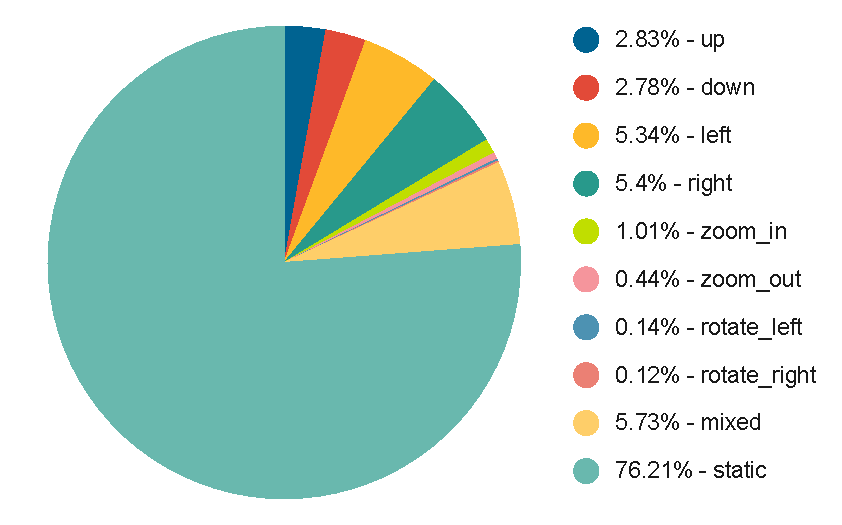
\includegraphics[width=\textwidth]{fig/23_03_07_Cholec80_motion_dist_no_title.pdf}
        \caption{Cholec80}
    \end{subfigure}
    \hfill
    \centering
    \begin{subfigure}[b]{0.49\textwidth}
        \centering
        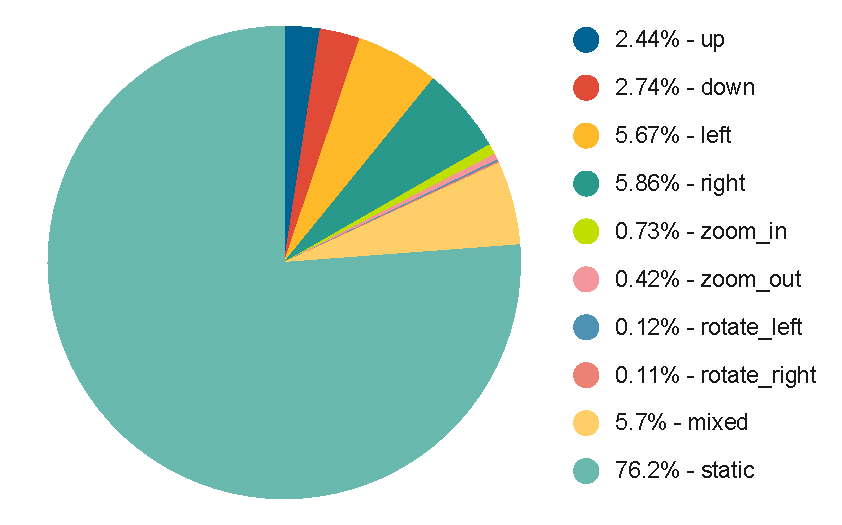
\includegraphics[width=\textwidth]{fig/23_03_07_HeiChole_motion_dist_no_title.pdf}
        \caption{HeiChole}
    \end{subfigure}
    % \begin{subfigure}[b]{0.49\textwidth}
    %    \centering
    %    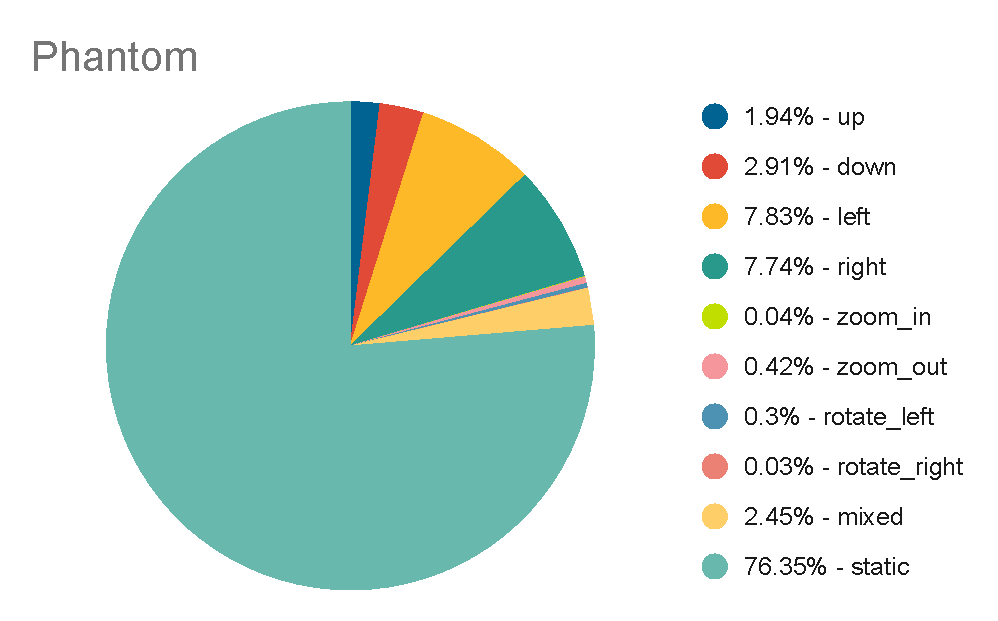
\includegraphics[width=\textwidth]{fig/23_03_07_Phantom_motion_dist.pdf}
    %    \caption{}
    % \end{subfigure}
    % \begin{subfigure}[b]{0.49\textwidth}
    %    \centering
    %    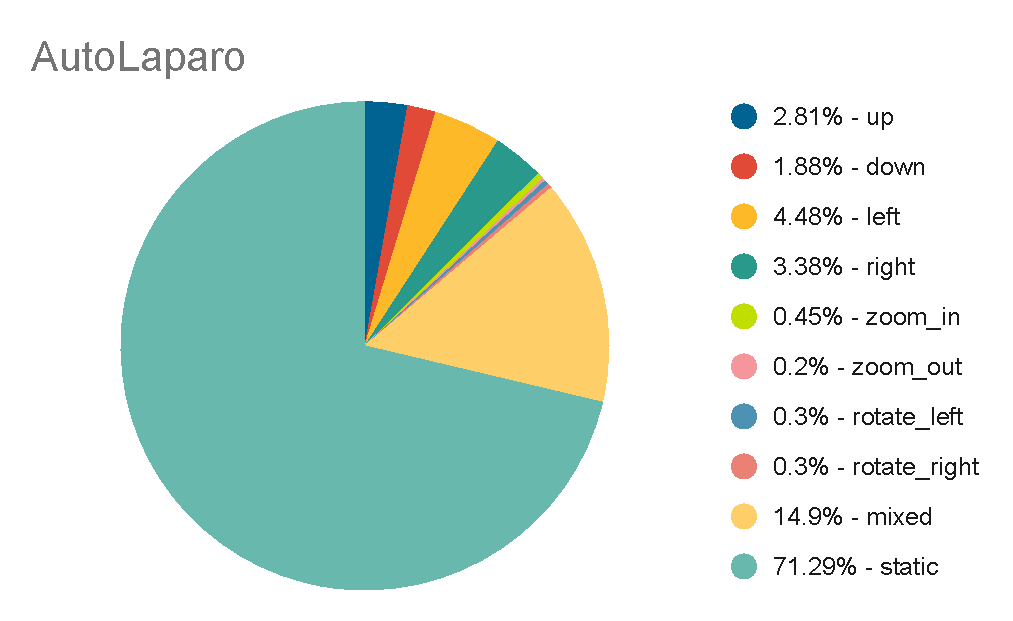
\includegraphics[width=\textwidth]{fig/23_03_07_AutoLaparo_motion_dist.pdf}
    %    \caption{}
    % \end{subfigure}
    \caption{Camera motion distribution, refer to \secref{c4:sec:camera_motion_estimator}. AutoLaparo: $2.81\%$ - up, $1.88\%$ - down, $4.48\%$ - left, $3.38\%$ - right, $0.45\%$ - zoom\_in, $0.2\%$ - zoom\_out, $0.3\%$ - rotate\_left $0.3\%$, - rotate\_right $14.9\%$ - mixed, $71.29\%$ - static.}
    \label{c4:fig:camera_motion_distribution}
\end{figure}

\subsubsection{Online Camera Motion Estimation}
The results of the online camera motion estimation are summarized in \tabref{c4:tab:estimation_speed}. The deep homography estimation with a Resnet34 backbone executes $11\times$ quicker and has the lowest \gls{gpu} memory footprint of the \gls{gpu} accelerated methods. This allows for efficient implementation of the proposed online camera motion estimation in \figref{c4:fig:training_pipeline}.

\begin{table}[htb]
    \caption{Memory footprint and execution time of different camera motion estimators, refer to \secref{c4:sec:online_camera_motion_estimation}.}
    \label{c4:tab:estimation_speed}
    \centering
    \resizebox{\textwidth}{!}{
        \begin{tabular}{lrrr}
            \toprule
            Method & Execution time [s] & Speed-up [a.u.] & Model / Batch [Mb] \\
            \midrule
            Resnet34 & $\mathbf{0.016 \pm 0.048}$ & $\mathbf{11.1}$ & $\mathbf{664} / \mathbf{457}$  \\
            \gls{loftr} \& \gls{ransac} & $0.178 \pm 0.06$ & $1.0$ & $669 / 2412$ \\
            \gls{surf} \& \gls{ransac} & $0.131 \pm 0.024$ & $1.4$ & NA \\
            \bottomrule
        \end{tabular}
    }
\end{table}

\subsection{Camera Motion Prediction}
The camera motion prediction results for all datasets are highlighted in \tabref{c4:tab:camera_motion_prediction}. It can be seen that significant improvements over the baseline are achieved on the Cholec80 and HeiChole datasets. Whilst the learned prediction performs better on average than the baseline, no significant improvement is found for the AutoLaparo dataset.

The displacement of the image center point under the predicted camera motion for AutoLaparo is plotted against the provided multi-class motion annotations and shown in \figref{c4:fig:autolapato_results}. It can be seen that the camera motion predictions align well with the ground truth labels.

% TODO: update cholec80 results here!
% TODO: move more sample to the appendix
\begin{table}[htb]
\caption{Camera motion predictor performance, refer to \secref{c4:sec:camera_motion_predictor_experiments}. Taylor baselines predict based on previous estimated motion, ResNets based on images.}
\label{c4:tab:camera_motion_prediction}
\centering
\resizebox{\linewidth}{!}{
\begin{tabular}{|l|l|lllll|}
\hline
\multirow{3}{*}{Dataset} & \multirow{3}{*}{\begin{tabular}[c]{@{}l@{}}Train Size\\ {[}Frames{]}\end{tabular}} & \multicolumn{5}{l|}{Mean Pairwise Distance {[}Pixels{]}}                                                                                                                                          \\ \cline{3-7} 
                         &                                                                                 & \multicolumn{2}{l|}{Taylor}                                                   & \multicolumn{3}{l|}{ResNet (proposed)}                                                                                              \\ \cline{3-7} 
                         &                                                                                 & \multicolumn{1}{l|}{$\mathcal{O}(1)$} & \multicolumn{1}{l|}{$\mathcal{O}(2)$} & \multicolumn{1}{l|}{$18$}                     & \multicolumn{1}{l|}{$34$}                     & $50$                     \\ \hline
Cholec80                 & $3.5e6$                                                                         & \multicolumn{1}{l|}{$27.2 \pm 23.1$}  & \multicolumn{1}{l|}{$36.4 \pm 31.2$}  & \multicolumn{1}{l|}{$\mathbf{14.8} \pm 11.7$} & \multicolumn{1}{l|}{$\mathbf{14.4} \pm 11.4$} & $\mathbf{14.4} \pm 11.4$ \\ \hline
HeiChole                 & $7.6e5$                                                                         & \multicolumn{1}{l|}{$29.7 \pm 26.4$}  & \multicolumn{1}{l|}{$39.8 \pm 35.9$}  & \multicolumn{1}{l|}{$\mathbf{15.8} \pm 12.5$} & \multicolumn{1}{l|}{$\mathbf{15.8} \pm 12.5$} & $\mathbf{15.8} \pm 12.5$ \\ \hline
AutoLaparo               & $5.9e4$                                                                         & \multicolumn{1}{l|}{$19.4 \pm 18.4$}  & \multicolumn{1}{l|}{$25.8 \pm 24.7$}  & \multicolumn{1}{l|}{$\mathbf{11.2} \pm 11.0$} & \multicolumn{1}{l|}{$\mathbf{11.3} \pm 11.0$} & $\mathbf{11.3} \pm 11.0$ \\ \hline
\end{tabular}
}
\end{table}

%cholec80 frames:
%4423520
%cholec80 train frames:
%3505700
%heichole frames:
%949469
%heichole train frames:
%763123
%phantom frames:
%7360
%phantom train frames:
%5888
%autolaparo frames:
%73500
%autolaparo train frames:
%58800

%mean estim
%mean pred

% cholec80 resnet 18
%$16.3 \pm 12.8$
%$8.1 \pm 6.3$

% cholec80 resnet 34
%$15.9 \pm 12.5$
%$8.1 \pm 6.4$

% cholec80 resnet 50
%$15.9 \pm 12.5$
%$7.8 \pm 6.1$

% heichole resnet 18
%$16.3 \pm 13.0$
%$6.2 \pm 4.5$

% heichole resnet 34
%$16.3 \pm 13.0$
%$7.3 \pm 5.4$

% heichole resnet 50
%$16.3 \pm 13.0$
%$6.5 \pm 4.3$

% autolaparo resnet 18
%$11.2 \pm 11.0$
%$1.0 \pm 0.3$

% autolaparo resnet 34
%$11.2 \pm 11.0$
%$1.2 \pm 0.4$

% autolaparo resnet 50
%$11.2 \pm 11.0$
%$1.1 \pm 0.7$

%phantom resnet 18
%$4.1 \pm 10.1$
%$5.8 \pm 4.6$

%phantom resnet 34
%$14.1 \pm 10.1$
%$3.3 \pm 0.6$

%phantom resnet 50
%$14.1 \pm 10.1$
%$4.0 \pm 1.6$

\begin{figure}[htb]
\centering
\begin{subfigure}[b]{0.49\textwidth}
    \centering
    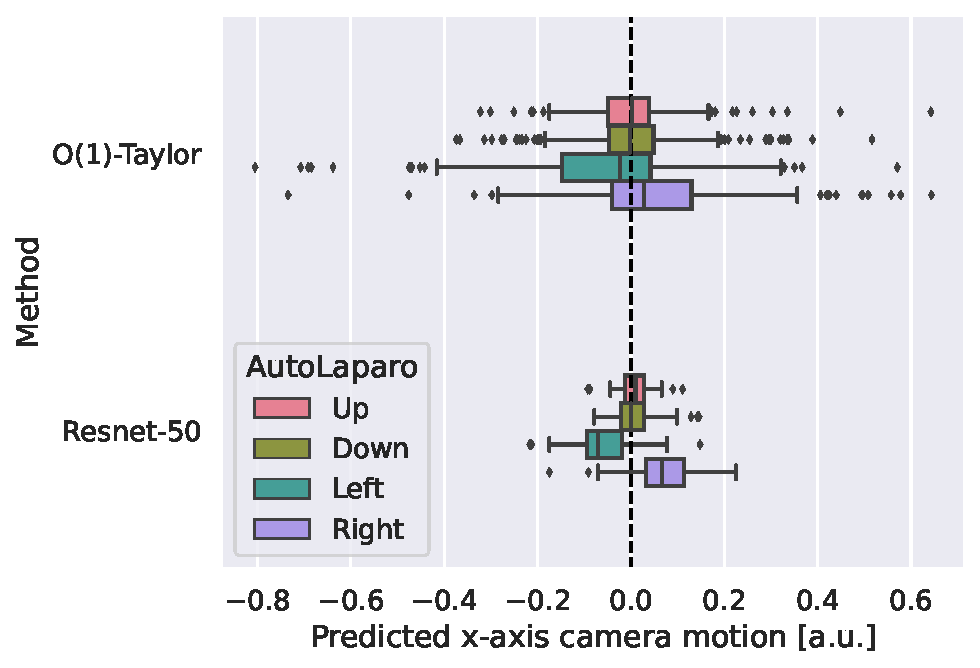
\includegraphics[width=\textwidth]{fig/23_03_07_autolaparo_cholec80_resnet50_duv_center_x.pdf}
    \caption{Predicted camera motion along x-axis, scaled by image size to $[-1, 1]$.}
    \label{c4:fig:autolaparo_results_a}
\end{subfigure}
\begin{subfigure}[b]{0.49\textwidth}
    \centering
    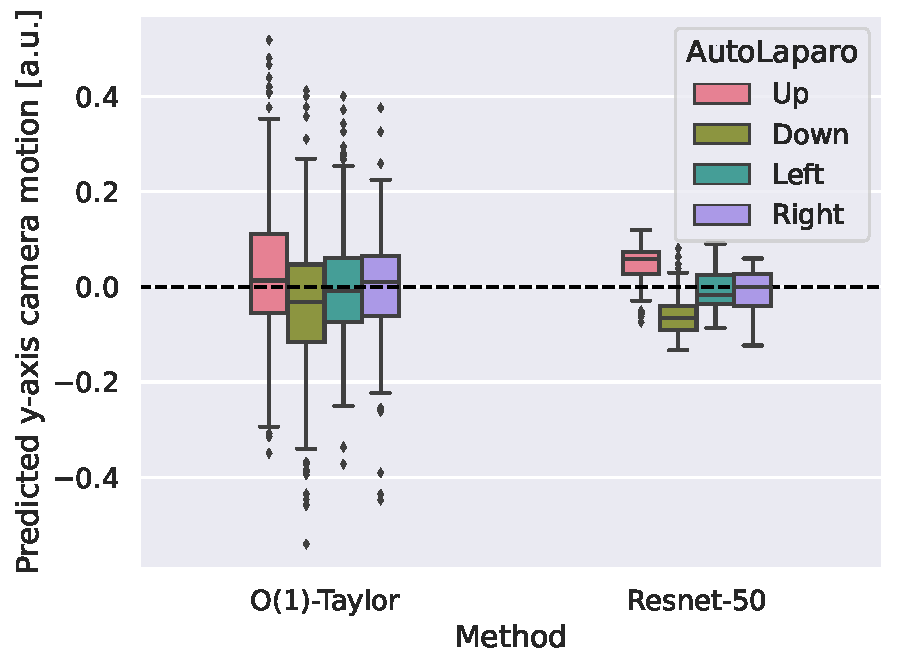
\includegraphics[width=\textwidth]{fig/23_03_07_autolaparo_cholec80_resnet50_duv_center_y.pdf}
    \caption{Predicted camera motion along y-axis, scaled by image size to $[-1, 1]$.}
    \label{c4:fig:autolaparo_results_b}
\end{subfigure}
\caption{Predicted camera motion on AutoLaparo, refer to \secref{c4:sec:camera_motion_predictor_experiments}. Camera motion predictor trained on Cholec80 with ResNet-50 backbone, see \tabref{c4:tab:camera_motion_prediction}. Shown is the motion of the image center under the predicted homography. Clearly, for videos labeled left/right, the center point is predicted to move left/right and for up/down labels, the predicted left/right motion is centered around zero (a). Same is observed for up/down motion in (b), where left/right motion is zero-centered.}
\label{c4:fig:autolapato_results}
\end{figure}

\begin{figure}[htb]
\centering
\includegraphics[width=\linewidth]{fig/23_03_09_blends_drawio_update.drawio.pdf}
\caption{Exemplary camera motion prediction, refer to \secref{c4:sec:camera_motion_predictor_experiments}. In the image sequence, the attention changes from the right to the left tool. We warp the past view (yellow) by the predicted homography and overlay the current view (blue). Good alignment corresponds to good camera motion prediction. Contrary to the baseline, the proposed method predicts the motion well. Data taken from HeiChole test set, ResNet-50 backbone trained on Cholec80, refer \tabref{c4:tab:camera_motion_prediction}.}
\label{c4:fig:predicted_camera_motion_sequence}
\end{figure}

% analysis should be done for all datasets!
% todo: surf or sift (kornia)
% loftr: 1078 nans


%Show a train / eval correlation matrix for every dataset, showing the improvements over baseline (motion continuation)
%\begin{table}[htb]
%    \caption{Figure showing the improvements over baseline. Trained / evaluated on different datasets.}
%    \label{c4:tab:my_label}
%    \centering
%    \begin{tabular}{ccccc}
%         Train / Eval & Cholec80 & HeiChole & Autolaparo & Phantom \\
%         Cholec80 & & & &  \\
%         HeiChole & & & &  \\
%         Phantom & & & &  \\
%    \end{tabular}
%\end{table}

%Show a figure of an image sequence with overlapped motion prediction for the best method
%\begin{itemize}
%    \item Identity
%    \item Continuation
%    \item Prediction
%\end{itemize}

\section{Conclusion and Future Work}
%In this work, we are the first
\paragraph{Results Discussion} To the best of our knowledge, this work is the first
to demonstrate that camera motion can indeed be learned from 
%publicly available
retrospective
videos of laparoscopic interventions,
with no manual annotation.
%simply
Self-supervision is achieved 
by harvesting image-motion correspondences using a camera motion estimator, see \figref{c4:fig:training_pipeline}. The camera motion predictor is shown to generate statistically significant better predictions over a baseline in \tabref{c4:tab:camera_motion_prediction} as measured using pseudo-ground-truth and on multi-class manually annotated motion labels from AutoLaparo in \figref{c4:fig:autolapato_results}. An exemplary image sequence in \figref{c4:fig:predicted_camera_motion_sequence} demonstrates successful camera motion prediction on HeiChole. These results were achieved through the key finding from \figref{c4:fig:camera_motion_distribution}, which states that most image sequences, i.e. static ones, are irrelevant to learning camera motion. Consequentially, we contribute a novel importance sampling method, as described in \secref{c4:sec:video_database_and_importance_sampling}. Finally, we hope that our open-source commitment will help the community explore this area of research further.

\paragraph{Limitations} A current limitations of this work is the preview horizon $M$ of length $1$. One might want to extend it for model predictive control. Furthermore, to improve explainability to the surgeon, but also to improve the prediction in general, it would be beneficial to include auxiliary tasks, e.g. tool and organ segmentation, surgical phase recognition, and audio. There also exist limitations for the camera motion estimator. The utilized camera motion estimator is efficient and isolates object motion well from camera motion, but is limited to relatively small camera motions. Improving the camera motion estimator to large camera motions would help increase the preview horizon $M$.

\paragraph{Future Work} In future work, we will execute this model in a real setup for investigating transferability. This endeavor is backed by \chapref{chap:robotic_endoscope}, which demonstrates how the learned homography could immediately be deployed on a robotic laparoscope holder. It  might prove necessary to fine-tune the presented policy through \gls{rlhf}.

